Б) Дано пространство $R$ функций, непрерывных на отрезке $[-\pi; \pi]$ со скалярным произведением $(f, g) = \int^\pi_{-\pi} f(t)g(t)dt$ и длиной вектора $\|f\| = sqrt{(f, f)}$.

Тригонометрические многочлены $P_n(t) = \frac{a_0}{2} + a_1 cost + b_1 sin t + \dots + a_n cos nt + b_n sin nt$, где $a_k, b_k$ - вещественные коэффициенты,
образуют подпространство $P$ пространства $R$.

Требуется найти многочлен $P_n(t)$ в пространстве $R$, минимально отличающийся от функции $f(t)$ - вектора пространства $R$.

Указание.
Требуется решить задачу о перпендикуляре: расстояние от $f\left(t\right)$ до $P_n\left(t\right)$ будет наименьшим,
если это длина перпендикуляра $h=f\left(t\right)-P_n\left(t\right)$, опущенного из точки $f\left(t\right)$ на подпространство $P$.
В этом случае, $P_n\left(t\right)$ будет ортогональной проекцией вектора $f\left(t\right)$ на $P$.
Таким образом, требуется найти координаты вектора $P_n\left(t\right)$ (коэффициенты многочлена) в заданном базисе $P$.
Если выбран ортонормированный базис, то эти координаты суть проекции вектора $f\left(t\right)$ на векторы данного базиса.

Проведите исследование:
\begin{enumerate}
	\item Проверьте, что система функций $\left\{1,\cos{t},\sin{t},\ldots\cos{n}t,\sin{n}t\right\}$ является ортогональным базисом подпространства $P$. Нормируйте систему.
	\item Найдите проекции вектора $f\left(t\right)$ (см. варианты) на векторы полученного ортонормированного базиса.
(На вектор $\left\{1\right\}$ найдите проекцию отдельно, а проекции на векторы вида $\left\{\cos{n}t\right\}$ и $\left\{\sin{n}t\right\}$ запишите формулами в зависимости от $n$. Воспользуйтесь свойствами интегралов от четных и нечетных функций на симметрично промежутке.)
	\item Запишите минимально отстоящий многочлен $P_n\left(t\right)$ с найденными коэффициентами (тригонометрический многочлен Фурье для данной функции).
	\item Изобразите (например, в Desmos) графики функции $f\left(t\right)$ и многочлена Фурье различных порядков $n$ (можно положить $n=5;10;15$).
	\item Сделайте вывод о поведении многочлена при росте его порядка.
\end{enumerate}

\[f\left(t\right)=-3t\]

\vspace{10mm}

\textbf{Решение.}

\begin{enumerate}
    \item Линейной комбинацией системы функций $\left\{1, cos t, sin t, ... cos nt, sin nt\right\}$ является пространство $P_n(t)$, значит эта система -- базис пространства. \\
        Этот базис ортогональный, для любых двух векторов $e_i, e_j (i \neq j)$ $(e_i, e_j) = 0$: \\
        \begin{trivlist}
        \item $(1, sin nt) = \int^\pi_{-\pi} sin nt dt = \frac{1}{n} cos n\pi - \frac{1}{n} cos n -\pi = 0$ (так как косинус чётная функция.)
        \item $(1, cos nt) = \int^\pi_{-\pi} cos nt dt = \frac{1}{n} sin n\pi - \frac{1}{n} sin n -\pi = \frac{2}{n} sin n\pi = 0$ (так как $n$ - целое число $sin n\pi = 0$)
        \item $(sin nt, cos mt) = \int^\pi_{-\pi} sin nt cos mt dt = \int^\pi_{-\pi} \frac{1}{2}(sin (n - m)t + sin (n + m)t dt) = \frac{1}{2} (\int^\pi_{-\pi} sin (n - m)t dt + \int^\pi_{-\pi} sin (n + m)t dt) = 0$ так как $\int^\pi_{-\pi} sin nt dt = 0$ при целом $n$ (см. выше).
        \end{trivlist}
        Нормируем базис. \\
        \begin{trivlist}
        \item $\sqrt{\int^\pi_{-\pi} 1^2 dt} = \sqrt{2\pi}$
        \item $\sqrt{\int^\pi_{-\pi} sin^2 nt dt} = \sqrt{\int^\pi_{-\pi} \frac{1 - cos 2nt}{2} dt} = \sqrt{\frac{2\pi}{2} - 0} = \sqrt{\pi}$
        \item $\sqrt{\int^\pi_{-\pi} cos^2 nt dt} = \sqrt{\int^\pi_{-\pi} \frac{1 + cos 2nt}{2} dt} = \sqrt{\frac{2\pi}{2} + 0} = \sqrt{\pi}$
        \end{trivlist}
        Итак, нормированный базис: ${\frac{1}{\sqrt{2\pi}}, \frac{sin t}{\sqrt{\pi}}, \frac{cos t}{\sqrt{\pi}}, ... \frac{sin nt}{\sqrt{\pi}}, \frac{cos nt}{\sqrt{\pi}} }$

    \item Чтобы найти проекции $f(t)$ на векторы базиса найдём скалярное произведение. \\
        \begin{trivlist}
        \item $a_0 = \int^\pi_{-\pi} \frac{1}{\sqrt{2\pi}} f(t) dt = \frac{1}{\sqrt{2\pi}} \int^\pi_{-\pi} -3t dt = \frac{-3}{\sqrt{2\pi}} \int^\pi_{-\pi} t dt = \frac{-3}{\sqrt{2\pi}} \cdot (\frac{\pi^2}{2} - \frac{{(-\pi)}^2}{2}) = 0$
        \item $a_n = \int^\pi_{-\pi} \frac{cos nt}{\sqrt{\pi}} f(t) dt = \frac{1}{\sqrt{\pi}} \int^\pi_{-\pi} -3t cos nt dt = \frac{-3}{\sqrt{\pi}} \int^\pi_{-\pi} t cos nb dt =$ \\
            $\int t n cos(nt) dt = \int t dsin(nt) = t sin(nt) - \int sin(nt) dt = \frac{t sin(nt) + \frac{1}{n} cos(nt)}{n} = \frac{nt sin(nt) + cos(nt)}{n^2}$ \\
            $= \frac{-3}{\sqrt{\pi}} \cdot (\frac{nt sin nt + cos nt}{n^2}\Big|^\pi_{-\pi}) = \frac{-3}{\sqrt{\pi}}((\frac{n\pi sin (n\pi)}{n^2} - \frac{-n\pi sin (-\pi n)}{n^2}) + (\frac{cos (n\pi)}{n^2}] - \frac{cos (-\pi n)}{n^2})) = \frac{-3}{\sqrt{\pi}}(0 + 0) = 0$
        \item $b_n = \int^\pi_{-\pi} \frac{sin nt}{\sqrt{\pi}} f(t) dt = \frac{1}{\sqrt{\pi}} \int^\pi_{-\pi} -3t sin nt dt = \frac{-3}{\sqrt{\pi}} \int^\pi_{-\pi} t sin nt dt =$ \\
            $\int t sin(nt) dt = \frac{1}{n} \int t d cod (nt) = -\frac{1}{n}(t cos(nt) - \int cos(nt) dt) = \frac{-(t cos(nt) - \frac{1}{n} sin(nt))}{n} = -(\frac{nt cos(nt) - sin(nt)}{n^2})$ \\
            $= \frac{3}{\sqrt{\pi}}(\frac{nt cos(nt) - sin(nt)}{n^2})\Big|^\pi_{-\pi} = \frac{3}{\sqrt{\pi}}((\frac{n \pi cos(n \pi)}{n^2} - \frac{-\pi n cos(-\pi n)}{n^2}) - (\frac{sin(\pi n)}{n^2} - \frac{sin(-\pi n)}{n^2})) = \frac{3}{\sqrt{\pi}}(\frac{2\pi n cos(n\pi) - 2sin(n\pi)}{n^2} = \frac{6n\pi cos(n\pi) - 6sin(n\pi)}{n^2\sqrt{\pi}}$
        \end{trivlist}
    \item Минимально отстоящий многочлен $P_n(t) = \sum^\infty_{n=1} (\frac{6n\pi cos(n\pi) - 6sin(n\pi)}{\sqrt{\pi}n^2} \frac{sin (nt)}{\sqrt{\pi}}) = \sum^\infty_{n=1} (\frac{6cos(n\pi)}{n} sin(nt)) = \sum^\infty_{n=1}(\frac{(-1)^n 6}{n} sin(nt))$
    \item 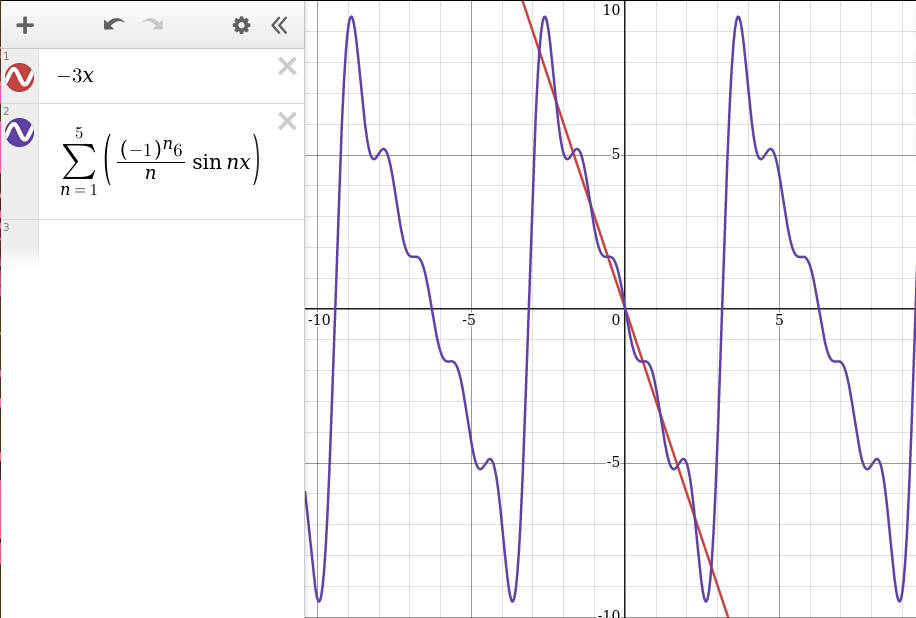
\includegraphics{images/1b_a} \\
        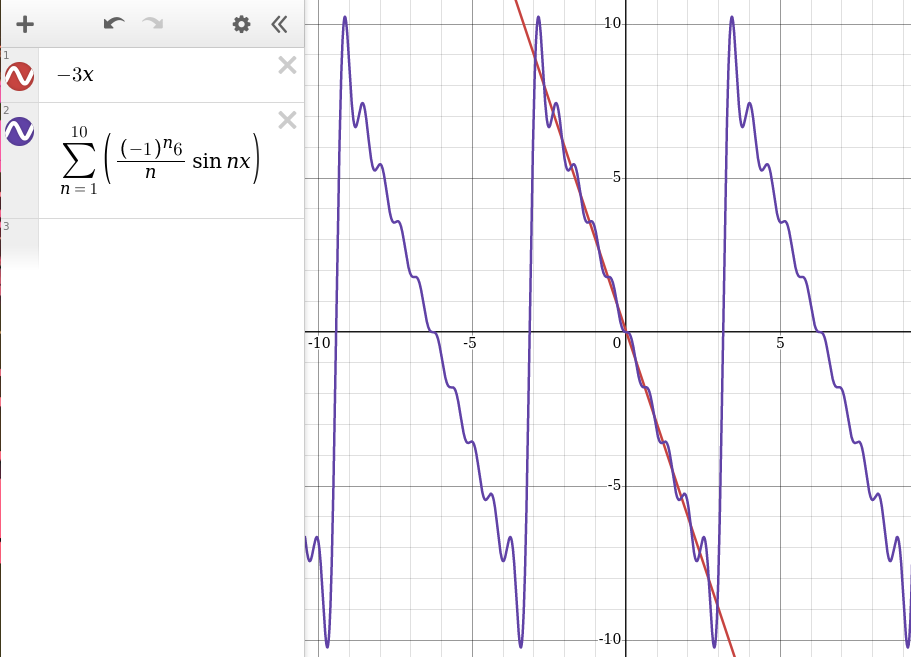
\includegraphics{images/1b_b} \\
        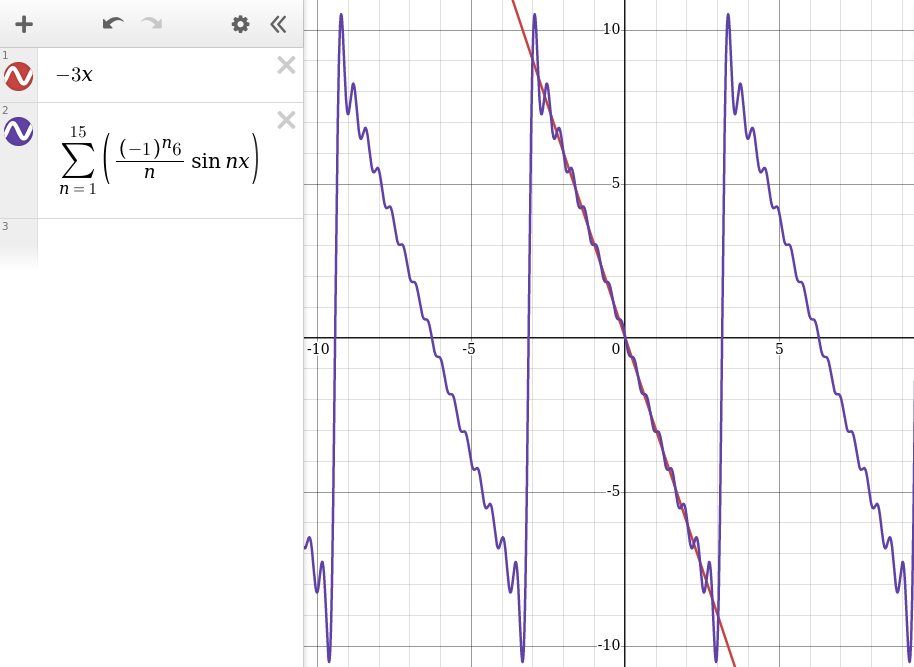
\includegraphics{images/1b_c}
    \item При росте порядка многочлен больше приближается к функции $f(t)$ на отрезке $[-\pi, \pi]$
\end{enumerate}
